%# -*- coding:utf-8 -*-
% Short topic proposal slides for Remote Sensing Geoscience Analysis

\PassOptionsToPackage{quiet}{fontspec}
\PassOptionsToPackage{dvipsnames}{xcolor}
\documentclass[10pt,aspectratio=169]{beamer}
\usepackage{zju_beamer}
\usepackage{booktabs}
\usepackage{array}
\graphicspath{{./figures/}}
\zjusectioncolor{blue}

\newcommand{\key}[1]{\textcolor{MidnightBlue}{\textbf{#1}}}
\newcommand{\imgfit}[2][0.95\linewidth]{%
  \IfFileExists{#2}{%
    \includegraphics[width=#1,height=0.58\textheight,keepaspectratio]{#2}%
  }{%
    \fbox{\parbox[c][0.22\textheight][c]{#1}{\centering\scriptsize
      图片文件暂未生成\\[0.35em]\texttt{\detokenize{#2}}}}%
  }%
}

\title[课程论文选题报告]{基于自编码器与 K-means 的\\Sentinel-2 多光谱遥感影像岩性聚类研究}
\subtitle{《遥感地学分析》课程论文选题报告}
\author[张项翌杰]{张项翌杰}
\institute[ZJU]{浙江大学}
\date{2026}

\begin{document}

\begin{frame}
  \titlepage
\end{frame}

\section{背景意义}
\begin{frame}{选题背景及意义}
  \begin{columns}[T,onlytextwidth]
    \begin{column}{0.50\linewidth}
      \begin{block}{研究背景}
        \begin{itemize}
          \item 干旱、半干旱裸露区植被覆盖低，基岩和蚀变信息暴露充分，是多光谱遥感岩性识别的典型应用场景。
          \item Sentinel-2 兼具可见光、近红外和短波红外波段，其中 SWIR 对含羟基蚀变矿物具有较强响应。
          \item 斑岩型铜矿区常发育绢英岩化、青磐岩化等热液蚀变带，可为遥感地质解释提供物理依据。
        \end{itemize}
      \end{block}
    \end{column}
    \begin{column}{0.46\linewidth}
      \begin{block}{研究意义}
        \begin{itemize}
          \item 在缺少可靠地面标签的条件下，探索无监督聚类用于岩性与蚀变候选区识别的可行性。
          \item 比较 PCA、浅层自编码器和堆叠自编码器的降维效果，分析非线性光谱表示的增益。
          \item 形成一套可复现、可迁移的 Sentinel-2 遥感地质分析流程。
        \end{itemize}
      \end{block}
    \end{column}
  \end{columns}
\end{frame}

\section{研究区}
\begin{frame}{研究区介绍}
  \begin{columns}[T,onlytextwidth]
    \begin{column}{0.38\linewidth}
      \begin{itemize}
        \item \key{位置：}新疆哈密市西南部土屋--延东地区，约 94.30$^\circ$E--94.70$^\circ$E、42.02$^\circ$N--42.32$^\circ$N。
        \item \key{构造背景：}位于东天山成矿带，是中国西北重要的斑岩型铜矿区之一。
        \item \key{地表条件：}气候干旱，植被稀疏，基岩裸露度高，适合开展光谱聚类与地质解译。
        \item \key{地质对象：}火山--沉积岩系、中酸性侵入岩及相关热液蚀变带。
      \end{itemize}
    \end{column}
    \begin{column}{0.58\linewidth}
      \centering
      \imgfit[\linewidth]{../data/processed/preview_geology_B12_B8A_B02.png}
      \vspace{0.3em}

      \scriptsize Sentinel-2 B12/B8A/B02 地质假彩色合成影像
    \end{column}
  \end{columns}
\end{frame}

\section{数据方法}
\begin{frame}{数据及方法}
  \small
  \begin{columns}[T,onlytextwidth]
    \begin{column}{0.42\linewidth}
      \begin{block}{数据来源}
        \begin{itemize}
          \item Sentinel-2A MSI Level-2A 地表反射率产品。
          \item 影像日期：2024-08-13；Tile：T46TFM。
          \item 使用 B02--B12 共 10 个可见光、近红外和短波红外波段。
          \item 统一至 20 m，并用 SCL 去除云、阴影、水体和无效像元。
        \end{itemize}
      \end{block}
    \end{column}
    \begin{column}{0.54\linewidth}
      \begin{block}{技术路线}
        \begin{enumerate}
          \item 构建 AOI 多光谱像元矩阵并进行 Z-score 标准化。
          \item 对比 Raw、PCA、Canonical AE、SAE 四组 K-means 流程。
          \item 用 Silhouette、DBI 和 CHI 评价聚类质量。
          \item 结合光谱响应与空间分布开展地质解释。
        \end{enumerate}
      \end{block}
      \vspace{0.2em}
      \centering
      \IfFileExists{../report/assets/image.png}{%
        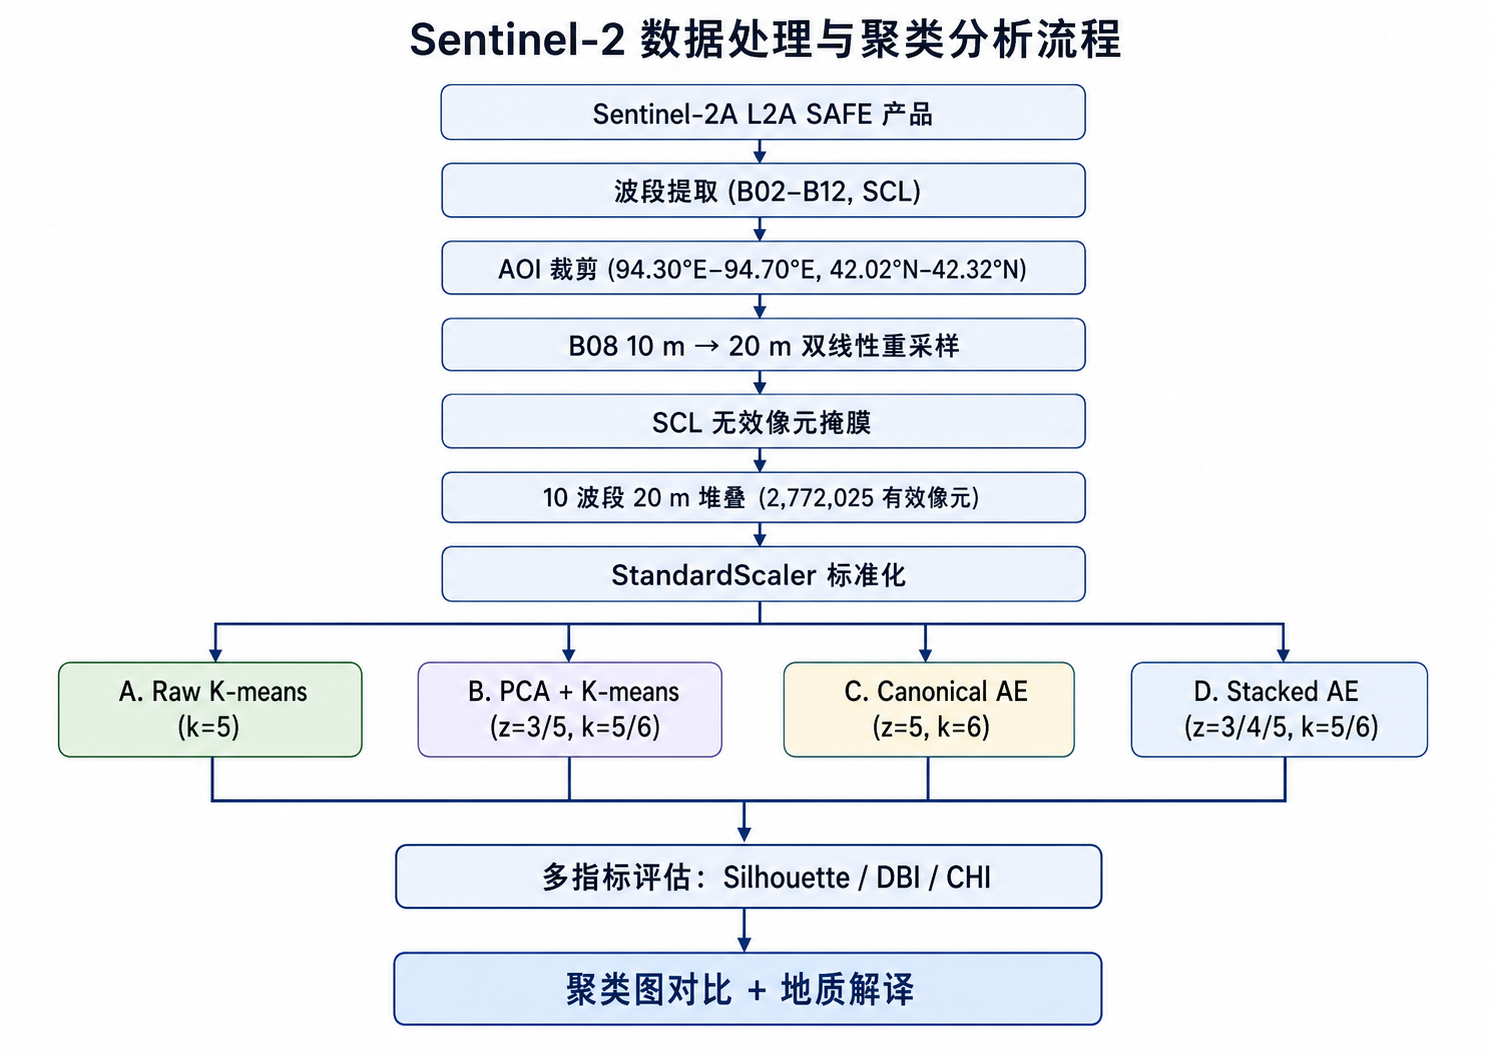
\includegraphics[width=0.82\linewidth,height=0.21\textheight,keepaspectratio]{../report/assets/image.png}%
      }{%
        \fbox{\parbox[c][0.14\textheight][c]{0.82\linewidth}{\centering\scriptsize
          图片文件暂未生成\\[0.25em]\texttt{../report/assets/image.png}}}%
      }
    \end{column}
  \end{columns}
\end{frame}

\section{可行性}
\begin{frame}{可行性分析及进度安排}
  \begin{columns}[T,onlytextwidth]
    \begin{column}{0.42\linewidth}
      \begin{block}{可行性分析}
        \begin{itemize}
          \item 数据可获得：Sentinel-2 L2A 产品公开、波段完整、研究区云量影响较小。
          \item 方法可实现：Python、rasterio、scikit-learn 与 PyTorch 可支撑预处理、降维、聚类和评价。
          \item 结果可解释：SWIR 波段对蚀变矿物敏感，可结合光谱比值与空间分布开展地质解释。
          \item 风险可控制：无地面标签时，将聚类结果定位为光谱推断和蚀变候选区，不直接等同正式地质图。
        \end{itemize}
      \end{block}
    \end{column}
    \begin{column}{0.54\linewidth}
      \scriptsize
      \begin{table}
        \centering
        \begin{tabular}{>{\raggedright\arraybackslash}p{0.18\linewidth}
                        >{\raggedright\arraybackslash}p{0.64\linewidth}}
          \toprule
          阶段 & 主要任务 \\
          \midrule
          第 1 周 & 完成 Sentinel-2 数据下载、AOI 裁剪、波段重采样和 SCL 掩膜。 \\
          第 2 周 & 构建 Raw、PCA、Canonical AE 和 SAE 四组聚类实验。 \\
          第 3 周 & 计算聚类指标，分析 bottleneck 维度、类别数量和空间结果。 \\
          第 4 周 & 完成光谱响应解释、图件制作和课程论文撰写。 \\
          \bottomrule
        \end{tabular}
      \end{table}
      \vspace{0.3em}
      \begin{block}{预期成果}
        \scriptsize
        形成研究区 Sentinel-2 多光谱聚类结果、方法对比评价表、蚀变候选区解释图，以及一篇结构完整的课程论文。
      \end{block}
    \end{column}
  \end{columns}
\end{frame}

\end{document}
